\chapter{ОБЗОР ПРОЕКТА}
\label{ch:ch1}


\section{Архитектура проекта}

Требования к окружению для текущего прототипа:
\begin{itemize}
\item OS: GNU/Linux
\item Наличие компилятора gcc
\end{itemize}

\vspace{5pt}
Проект выполнен как динамическая библиотека \verb|libec.so| и небольшая утилита \verb|ecc| использующая ее.

Следующая диаграмма[\ref{arch:diag}] иллюстрирует архитектуру проекта:

\begin{figure}[h!]
    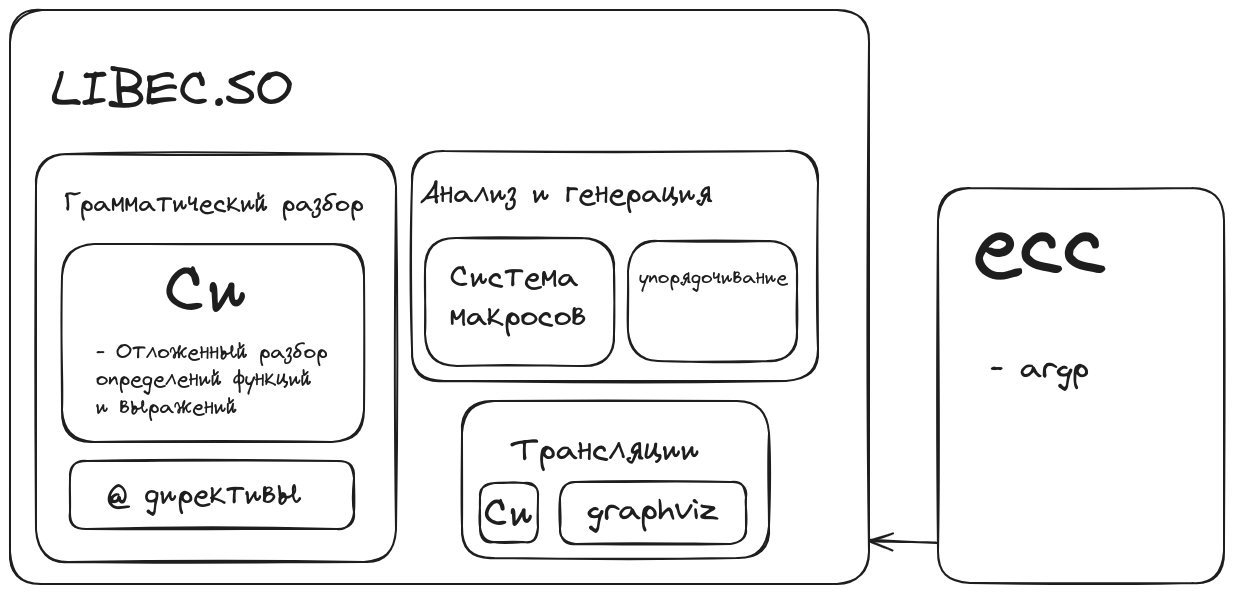
\includegraphics[width=\textwidth,height=0.8\textheight,keepaspectratio]{arch-diag.png}
    \centering
    \caption{Архитектура проекта}
    \label{arch:diag}
\end{figure}

Библиотека \verb|ec.so| имеет высокоуровневый интерфейс, реализованный в виде методов единицы трансляции(в коде \verb|C_TranslationUnitData|).
Данный интерфейс организует функционал библиотеки в виде проходов и их композиций.
Каждый проход это отдельный этап трансляции. 
Подробно каждый проход рассматривается в следующей главе[\ref{passes}].

Так как синтаксически ЕС это небольшая надстройка над языком Си, 
то парсер Си(и некоторые другие проходы, например трансляции) библиотеки ec.so может быть использован отдельно от языка EC.

Интерфейс утилиты \verb|ecc| подробно описан далее[\ref{details:ecc-cli}].

% Данный функционал предоставлен пользователю для решения задач метапрограммирования: предобработки, умной компиляции, и др.

% Поверх стандартного функционала разбора языка Си в библиотеку добавлено синтаксическое расширение языка: Extended C
% Которое может быть использовано пользователем для разметки программного кода с целью последующей его обработки, что продемонстрировано далее[\ref{use-ex:code-gen}]

\section{Обзор языка EC}

EC представляет собой слой предобработки языка Си, повышающий его эргономику.
EC реализует систему директив, выполняющих функцию разметки кода, с возможностью последующей их интерпретации.

В реализованном на данный момент прототипе представлены следующие директивы:
\begin{itemize}
\item \verb|@derive(identifier)| применяет к следующему за директивой определению макро-функцию вывода указанную в \verb|identifier|
\item \verb|@derive_macro(identifier)| регистрирует следующее за директивой определение функции как макро-функцию вывода адресуемую с помощью \verb|identifier|
\item \verb|@post_include(string-literal)| при трансляции в язык Си заменяется на обычную директиву препроцессора \verb|#include string-literal|
\end{itemize}

С помощью данных директив в EC реализованна система макросов. На данный момент реализованны только макросы вывода (derive macro).
Макросы(или макро-функции) вывода это функции, генерирующие блок кода, оформленного в виде элемента AST единицы трансляции, по данному AST определению.

Все макро-функции вывода должны иметь следующий интерфейс:
\begin{lstlisting}[language=C]
typedef ProcMacroError
DeriveMacroFn(C_TranslationUnitData *, C_Ast_Decl *, C_Ast_TranslationUnit **);
\end{lstlisting}

Макро-функции должны находиться в отдельном файле, т.к. библиотека макро-функций является отдельной единицей трансляции.
При компиляции \verb|ecc| сначала компилирует все макро-функции как динамическую библиотеку, линкуя ее с основной библиотекой \verb|libec.so|, затем динамически подгружает ее в свое виртуальное адресное пространство, после чего возможен вызов данных функций.
Подробнее этот процесс описан далее[\ref{pass:macros}].

Зачастую бывает нецелесообразно генерировать код заполняя AST структуру вручную, альтернативой этому на данный момент служит написание генерируемого кода в виде строки,
используя вспомогательный примитив \verb|StringFormatter|, рассмотренный далее[\ref{primitives:formatter}], и последующий его грамматический разбор.
Функционал грамматического разбора, приведенный в заголовочном файле \verb|proc_macro.h| использует библиотеку \verb|libec.so|.

Рассмотрим пример макро-функции вывода:
\lstinputlisting[language={C},caption={macros.ec},label={use-ex:macro-file}]{listings/ch1/use-ex/ex_macro.ec}

Данная макро-функция генерирует функции отладочного форматирования для структур языка Си.
Вспомогательная функция \verb|gen_dbg_fmt_fmt| генерирует текст программы, а основная выполняет функцию обработки ошибок и грамматического разбора текста сгенерированной программы.
Получившийся в процессе генерации AST элемент(единица трансляции) возвращается компилятору, выполняющему дальнейшие преобразования.

Так например из следующего определения структуры языка Си
\begin{lstlisting}[language=C]
struct Foo {
    int x;
    int y;
    int z;
};
\end{lstlisting}

генерируется следующая функция отладочного форматирования
\begin{lstlisting}[language=C]
FmtError Foo_dbg_fmt(Foo *self, StringFormatter *fmt, void *_) {
    TRY(string_formatter_write_fmt(fmt, S("Foo:%+\nx: %d\ny: %d\nz: %d\n%-"), self->x, self->y, self->z));
    return FMT_ERROR(OK);
}
\end{lstlisting}

печатающая структуру \verb|Foo| со значениями полей: \verb|x=3, y=4, z=5| следующим образом
\begin{lstlisting}[language=C]
Foo:
    x: 3
    y: 4
    z: 5
\end{lstlisting}

В примере[\ref{use-ex:macro-file}] функция \verb|gen_dbg_fmt| помечена директивой\newline \verb|@derive_macro(DebugFormat)|, регистрирующей ее в базе макро-функций компилятора под именем \verb|DebugFormat|.
Далее данная функция может быть применена к определению языка Си с помощью родственной директивы \verb|@derive(DebugFormat)|.

Пример использования данной макро функции приведен далее[\ref{use-ex:code-gen}].

\section{Пример программы на EC}
\label{use-ex:simple}

Для демострации языка приведем следующую простую программу[\ref{use-ex:simple-souce}]:
\begin{lstlisting}[language=C, caption={simple.ec}, label={use-ex:simple-souce}]
@post_include("demo.h")

struct A {
    B b;
};

int main() {
    ctx_init_default();
    
    g_x = 5;
    foo(g_x);

    ctx_deinit();
}

struct B {
    A *ap;
    C c;
};
struct C {
    B *bp;
};

int g_x;

void foo(int x) {
    print_fmt(S("x: %d\n"), x);
}
\end{lstlisting}

Данная программа не скомпилируется компилятором Си, даже если заменить директиву в начале файла на обычный \verb|#include "demo.h"|.
Так например \verb|gcc| выдает ошибку[\ref{use-ex:simple-gcc-err}]:

\begin{lstlisting}[language=Bash, caption={Ошибка gcc}, label={use-ex:simple-gcc-err}]
error: unknown type name ‘B’
...
error: ‘g_x’ undeclared
...
\end{lstlisting}

Связано это с тем, что в Си зависимости разрешаются линейно(сверху вниз), 
т.е. когда компилятор увидел имя \verb|B| в структуре \verb|A| он \textquote{запаниковал}, так как ранее(выше) это имя не приводилось.

В EC внешние определения могут идти в любом порядке. Под внешними в данном случае понимается те, 
что приведены непосредственно в корне файла, не содержатся в определении функции(или составного утверждения).

Также в примере используются \textquote{голые} имена структур, тогда как в Си при объявление, 
приведенном в примере, имена структур(и других составных типов) надо приводить с префиксом, например \verb|struct A|.
EC избавляет пользователя от данной необходимости.
% EC вставляет \verb|typedef struct A A;| в генерируемый Си файл, что объ

Подробнее об ток, как EC преобразует внешние определения см. далее[\ref{pass:ordering}].

Скомпилируем данную программу компилятором \verb|ecc| с помощью команды:
\begin{lstlisting}[language=Bash]
$ ecc simple.ec -o simple
\end{lstlisting}

Запуская полученный файл, получаем ожидаемый результат:
\begin{lstlisting}[language=Bash]
$ ./simple
x: 5
\end{lstlisting}


\section{Пример генерации кода}
\label{use-ex:code-gen}

Продемонстрирую как выглядит процесс работы с системой макросов языка EC.

Допустим у вас есть файл[\ref{use-ex:source-file}] \verb|example.ec| с исходным кодом EC, который вы хотите скомпилировать, предварительно применив макро-функции, определенные по требованиям системы макросов в отдельном файле, назовем \verb|macros.ec|.
Пусть содержание файла совпадает с приведенном ранее в обзоре языка EC[\ref{use-ex:macro-file}].

% \lstinputlisting[language={C},caption={example.ec},label={use-ex:source-file}]{listings/ch1/use-ex/ex4.ec}
\begin{lstlisting}[language=c, caption={example.ec}, label={use-ex:source-file}]
@post_include("parsing/c/parsing.c")

@derive(DebugFormat)
struct Foo {
    int x;
    int y;
    int z;
};

@derive(DebugFormat)
struct Bar {
    int x;
    int y;
    int z;
};

int main() {
    ctx_init_default();

    Foo foo = (Foo) {
        .x = 3,
        .y = 4,
        .z = 5,
    };
    dbgp(Foo, &foo);

    Bar bar = (Bar) {
        .x = 6,
        .y = 7,
        .z = 8,
    };
    dbgp(Bar, &bar);

    ctx_deinit();
}
\end{lstlisting}

Данный файл состоит из определений двух структур(\verb|Foo| и \verb|Bar|), для которых автоматически генерируются функции отладочного форматирования посредством директивы \verb|@derive|.
С помощью макроса препроцессора Си \verb|dbgp|, подхватывающего данные функции форматирования, печатаем в консоль значения содержащиеся в структурах.

Итак содержимое файла \verb|example.ec| компилирует с применение макросов командой:
\begin{lstlisting}[language=Bash]
$ ecc -p macro.ec example.ec -o example
\end{lstlisting}

Запуская полученный файл, получаем напечатанные структуры:
\begin{lstlisting}[language=Bash]
$ ./example
Foo:
    x: 3
    y: 4
    z: 5

Bar:
    x: 6
    y: 7
    z: 8
\end{lstlisting}

В этом примере используются всего две структуры, когда кол-во подобных объектов возрастает, возрастает и эффективность данной системы.

Результат работы данной системы можно увидеть, если посмотреть сгенерированный промежуточный файл[\ref{use-ex:c-tmp}] с кодом языка Си.

\lstinputlisting[language={C},caption={example\_tmp.c},label={use-ex:c-tmp}]{listings/ch1/use-ex/ex4_tmp.c}

Подробнее данный процесс будет рассмотрен далее[\ref{pass:ordering}, \ref{pass:macros}]

\section{Сравнение с другими языками}
Рассмотрим решения в других языках программирования:

\begin{enumerate}
% \item\label{langcmp:c} Сравнение с языком C:\brake - line was streched
\item\label{langcmp:c} Сравнение с языком C:\newline
Си - довольно старый системный язык, разработанный Деннисом Ритчи еще в 70х годах прошлого столетия, однако активно применяется и по сей день, среди ярких примеров применения: ядро операционной системы Linux, различные embedded системы.
С тех пор вышло несколько версий языка, среди них самая последняя C23, она же использовалась при написании данной работы.
Си это язык со слабой статической типизацией, благодаря чему во многом представляет собой высокоуровневый ассемблер.

В данной работе реализованно небольшое синтаксическое расширение языка Си, представляющее собой своеобразную систему разметки, семантическая часть языка не тронута.
Улучшена эргономика языка за счет автоматического упорядочивания определений(структурный элементов языка) в порядке зависимостей, что было продемонстрировано выше[\ref{use-ex:simple}].



\item\label{langcmp:cpp} Сравнение с языком C++:\newline
C++ является системным языком программирования, доминирующим на рынке в сфере ПО с требованиями по производительности. 
C++ несомненно объемный язык, в нем присутствуют такие системы как:
\begin{itemize}
\item подмножество языка Си
\item расширенная система типов Си
\item статический полиморфизм на перегрузке функций
\item система шаблонов, которая применяется как для статического полиморфизма, так и для метапрограммирования
\item система пространств имен
\item ООП система с возможностями динамического полиморфизма
\end{itemize}

Все это многообразие делает процесс разрешения имен в C++ очень сложным. 
Некоторые системы C++, например система виртуальных функций, через которые реализуется динамический полиморфизм, 
не дают пользователю контроля на тем как именно виртуальные таблицы располагаются в памяти.

В тех случаях когда этот контроль важен(например при динамической подгрузке и линковке библиотек) зачастую вовсе отказываются данной подсистемы и реализуют аналогичную в стиле Си остальными средствами языка C++.

В философии EC подобные подсистемы должны быть реализованы в виде пользовательских библиотек, с улучшенной эргономикой посредством макросов, позволяющей расширять язык средствами самого языка.
Так разработчик имеет максимальный контроль над используемыми инструментами, неограничен в их доработке и настройке под конкретный проект.

Так как Си является частичным подмножеством языка C++, то пункты приведенные выше[\ref{langcmp:c}] также применяются.

Для C/C++ существует компилятор Clang, у которого frontend вынесен в качестве библиотеки, однако данный компилятор заточен больше на C++, что существенно усложняет Ast, 
поэтому было принято решения написать свой минималистичный frontend для Си.



\item\label{langcmp:rust} Сравнение с языком Rust:\newline
Rust является системным языком программирования с развитой системой типов, позволяющей проводить глубокий статический анализ, в частности анализ и выведение времени жизни переменных, 
что используется при обнаружение ошибок связанных с владением памятью, таких как
\begin{itemize}
\item использование после освобождения памяти(use-after-free)
\item повторное освобождение памяти(double-free) 
\item утечка памяти(memory-leak)
\end{itemize}


В языке Rust представлена система\cite{rust-proc-macro} процедурных макросов, схожая с системой, выполненной в данной работе.
В Rust также есть \verb|Derive| макросы(макросы вывода) дающие такой же функционал, что и \verb|@derive| директивы представленные в данной работе.
Макросы в Rust также компилируются в отдельной единице трансляции(\verb|crate| в терминологии Rust).

Отличие состоит в том, что макросы в Rust работают на уровне токенов(лексем), тогда как макросы в данном проекте работают на уровне элемента AST подобно языку Julia[\ref{langcmp:julia}].

Для сравнения привожу заголовки функций макросов из обоих языков[\ref{langcmp:rust:rust_pmh}, \ref{langcmp:rust:ec_pmh}]:


\begin{lstlisting}[language=C, caption={Заголовок процедурного макроса Rust}, label={langcmp:rust:rust_pmh}]
#[proc_macro_derive(AnswerFn)]
pub fn derive_answer_fn(_item: TokenStream) -> TokenStream;
\end{lstlisting}

\begin{lstlisting}[language=C, caption={Заголовок процедурного макроса EC}, label={langcmp:rust:ec_pmh}]
@derive_macro(DebugFormat)
ProcMacroError
gen_dbg_fmt(C_TranslationUnitData *data, C_Ast_Decl *decl, C_Ast_TranslationUnit **out_node);
\end{lstlisting}

Где \verb|TokenStream| - тип потока токенов в языке Rust.

Генерация кода, путем заполнения AST напрямую - трудоемкий и нецелесообразный подход.
Поэтому в Rust есть функционал "цитирования" кода, предоставляемый пакетом(\verb|crate|) \verb|quote|\cite{rust-quote}.
Данный пакет предоставляет макро-функцию \verb|quote!|, реализованную как декларативный макрос(еще один вид макросов) самого языка Rust.

Пример цитирования кода:
\begin{lstlisting}[language=C, caption={Заголовок процедурного макроса Rust}, label={langcmp:rust:rust_quote}]
let varname = format_ident!("_{}", ident);
quote! {
    let mut #varname = 0;
}
\end{lstlisting}

Так мы можем писать генерируемый код, как если бы писали код обычной функции. К тому же есть возможность подстановки выражений из локальных переменных.
Опять же все это работает на уровне токенов, т.е. макро-функция \verb|quote| возвращает поток токенов, получая блок текста(программы).

В моей работе на данный момент единственный целесообразный способ генерации кода это генерация его в виде строки, с последующим грамматическим разбором, как показано ранее в примере[\ref{use-ex:code-gen}].

Также в EC макро-функциях на вход приходит разобранный AST элемент, тогда как в Rust приходит простой поток токенов.
Для анализа и обработки программы нужно грамматически разобрать его, для этого в Rust есть пользовательский пакет \verb|syn|\cite{rust-syn}, реализующий парсер языка Rust.

Также как в EC порядок следования определений в тексте программы не играет роли в Rust.

\item\label{langcmp:julia} Сравнение с языком Julia:\newline
Язык Juila это скриптовый язык с динамической типизацией подобно языку Python. Система JIT(just-in-time, точно в срок)-компиляции, использующая LLVM\cite{llvm} позволяется данному языку компилироваться напрямую в машинный код, 
что благодаря оптимизациям LLVM позволяет добиться производительности близкой к производительности языка Си.

Язык Julia имеет похожую систему макро-функций\cite{julia-meta}, с единственным отличием, что в Julia макро-функции могут идти вперемешку с остальными. 
Связано это с тем, что в Julia определения функций интерпретируются линейно по ходу текста программы, в EC определения интерпретируются вне зависимости от порядка их следования в тексте.

Синтаксически макросы в Julia почти полностью совпадают с директивами EC.

\item\label{langcmp:zig} Сравнение с языком Zig:\newline
Zig это относительно молодой язык программирования, стремящийся занять туже нишу, что C/C++. 
Также как в Rust продвинутая система типов позволяет этому языку предотвратить множество ошибок при работе с памятью на этапе компиляции.
Если ставить в соответствие Zig, Rust и C, C++, то Zig будет ближе к C, а Rust будет ближе к C++.

В языке Zig метапрограммирование выполнено с помощью функционала \verb|comptime| - позволяющего выполнять код во время компиляции и функционала рефлексии, 
позволяющего получить информацию о типе в виде \verb|comptime| структуры, что предоставляет гибкий интерфейс для расширения возможностей компилятора, не прибегая 
к сторонним утилитам, а также для метапрограммирования, не взаимодействуя с AST напрямую.
\end{enumerate}